\section{Primitives}\label{csx_primitive} 

After defining the property of interest into 
\matv{CSX}\phantomsection\label{CSX}, user has to assign a primitive to that property by 'matching' the name of property and primitive. A warning will occur if a property without primitive has been added \matv{CSX}\phantomsection\label{CSX}. An error message will pop up if a primitive without property specification has been assigned. This primitive can be defined in either cartesian or cylindrical coordinate. The following primitives function are defined and can be added into \matv{CSX}\phantomsection\label{CSX}:   
\begin{enumerate}
\item{Point} (refer to \ref{point})
\item{Box} (refer to \ref{box})
\item{Cylinder} (refer to \ref{cylinder})
\item{CylindricalShell}(refer to \ref{cylindershell})
\item{Sphere}(refer to \ref{sphere})
\item{SphericalShell}(refer to \ref{sphereshell})
\item{Curve}(refer to \ref{curve})
\item{Wire}(refer to \ref{wire})
\item{Polygon}(refer to \ref{polygon})
\item{2D polygon}(refer to \ref{2dpoly})
\end{enumerate}

\subsection{General primitive setup} \phantomsection\label{prim_setup}
To add a primitive into \hyperref[CSX]{\matv{CSX}}, it has a common structure as shown below:

\begin{FontDescr}{Syntax:}
\begin{lstlisting} 
CSX=Add<..primitive..>(CSX,propName,prio...)
\end{lstlisting} 
\end{FontDescr}

\begin{FontDescr}{Description:}
\matv{CSX} 
\phantomsection \label{CSX}
\begin{myindentpar}
\matv{CSX} describes geometrical objects and their physical or non-physical properties in .xml file.
\end{myindentpar}

\matv{propName} 
\begin{myindentpar}
\texttt{name} is given by user and must be matched with that is mentioned in the \texttt{Add<...property...>}.Refer to \hyperref[subsection_gprop_setup]{subsection 4.1.1}.  
\end{myindentpar}

\matv{prio} 
\begin{myindentpar}
Priority of primitive.    
\end{myindentpar}
\end{FontDescr}




\subsection{Point} \phantomsection\label{point}
\input{chapter/SEC_CSXCAD_Setup/prim_point}

\subsection{Box} \phantomsection\label{box}
User can define a cube(3D),rectangular cube(3D),plane(2D),line(1D) or a point with this primitive by defining its lower-left-bottom and upper-right-top edge.

\begin{FontNameFunct}{AddBox()}
\end{FontNameFunct} 

\begin{FontDescr}{Purpose:}
Add a box to \matv{CSX}\phantomsection\label{CSX} with predefined property in either cartesian- or cylindrical- coordinate. The name of property and primitive must match.  
\end{FontDescr}

\begin{FontDescr}{Syntax:}
\begin{lstlisting} 
 CSX = AddBox(CSX, propName, prio, start, stop, varargin)
\end{lstlisting}
\end{FontDescr}

\begin{FontDescr}{Description:}

\begin{FontPara}{propName} \phantomsection \label{prim_Name}
Primitive Name which must be the same with that mentioned in the \texttt{Add<...property...>}. Refer to \hyperref[subsection_gprop_setup]{subsection 4.1.1}.
\end{FontPara}

\begin{FontPara}{start}
Start coordinate of a box.(vector)
\end{FontPara}

\begin{FontPara}{stop}
Stop coordinate of a box.(vector)
\end{FontPara}

\end{FontDescr}

\begin{FontDescr}{Optional Arguments:} \phantomsection \label{prim_transform}
\begin{FontPara}{'Transform'}
Transformation of a primitive in 3D material/metal discretisation.
\begin{itemize}
\item\textcolor{varcol}{'Scale'}: scale the model with scale factor.\\ For example,'1,1,2': the z-dimension is scaled with 2. 

\item\textcolor{varcol}{'Rotate$\_$X'}:  Rotate the structure around x-axis.\\ For example, pi/4: structure will be rotated $45^{0}$. \\'Rotate$\_$Y' and 'Rotate$\_$Z' are available too.  

\item\textcolor{varcol}{'Translate'}: Translate the structure with defined distance.\\For example,'0,0,100': model will be z-direction shifted to 100 drawing unit.
\end{itemize}
\end{FontPara}
\end{FontDescr}

\begin{FontDescr}{Examples:}

\begin{lstlisting}
 CSX=InitCSX('CoordSystem',0);
 CSX = AddMetal(CSX,'metal'); 
 CSX = AddBox(CSX,'metal',10,[0 0 -100],[100 100 0]);
\end{lstlisting} 

A metal box has been defined in Cartesian coordinate and has size 100x100x100 in drawing unit.

\begin{lstlisting}
CSX=InitCSX('CoordSystem',0);
CSX = AddMetal(CSX,'metal'); 
CSX = AddBox(CSX,'metal',10,[0 0 -100],[100 100 0],'Transform', {'Rotate_Z', pi/4});  
\end{lstlisting}  
The box is then rotated $45^{0}$ around z-axis.   


The following example will describe the box definition in cylindrical coordinate: 

\begin{lstlisting} 
 CSX=InitCSX('CoordSystem',1);
 radius=100;
 mesh_factor=[1 1/radius 1];
 CSX = AddMetal(CSX,'metal'); 
 CSX = AddBox(CSX,'metal',10,[0 0 -100].* mesh_factor,[100 100 0].* mesh_factor);
\end{lstlisting}
The metal box has been transformed into a sector of a circle with radius=100. The dimension of a box: 
\begin{itemize}
\item x=0 $\rightarrow$ 100    $\Rightarrow $   r=0 $\rightarrow$ 100

\item y=0$\rightarrow$ 100     $\Rightarrow $   a=0 $\rightarrow$ 100/radius(=1 radian)

\item z=-100$\rightarrow$ 0    $\Rightarrow $   z=-100 $\rightarrow$ 0
\end{itemize}            
\end{FontDescr}

\begin{figure}[hbt]
\centering
\subfloat[In Cartesian coordinate]{\includegraphics[width=0.39\textwidth]{svg/box_carteco.pdf}}
\subfloat[In Cylindrical coordinate]{\includegraphics[width=0.4\textwidth]{svg/box_cylinderco.pdf}}
\caption{Top view of the box in Cartesian coordinate and Cylindrical coordinate.}
\label{fig:primBox}
\end{figure}



\subsection{Cylinder } \phantomsection\label{cylinder}
Introduce a cylinder into\hyperref[CSX]{\matv{CSX}} with predefined matlab function \texttt{AddCylinder}.

\begin{FontNameFunct}{AddCylinder()}
\end{FontNameFunct}

\begin{FontDescr}{Purpose:}
Define cylinder with its axis(where it extends) and radius and assign a property to it. 
\end{FontDescr}

\begin{FontDescr}{Syntax:}
\begin{lstlisting} 
 CSX = AddCylinder(CSX, propName, prio, start, stop, rad, varargin)
\end{lstlisting}
\end{FontDescr}

\begin{FontDescr}{Description:}

\begin{FontPara}{propName}
Refer to \hyperref[prim_Name]{propName} in \texttt{AddBox}. 
\end{FontPara}

\begin{FontPara}{start}
A vector represents start point of cylinder axis.  
\end{FontPara}

\begin{FontPara}{stop}
End point of cylinder axis(vector). Extend in the same direction as start point.  
\end{FontPara}

\begin{FontPara}{rad}
Radius of cylinder. In drawing unit. 
\end{FontPara}
\end{FontDescr}

\begin{FontDescr}{Optional Arguments:}
The standard trasformation (rotation,translation,scaling) mentioned in  \hyperref[prim_transform]{\matv{'Transform'}} of \texttt{AddBox}.  
\end{FontDescr}

\begin{FontDescr}{Examples:}

\begin{lstlisting} 
CSX=AddMaterial(CSX,'phantom');
CSX=SetMaterialProperty(CSX,'phantom','Epsilon',75.5,
'Kappa',0.438,'Density',1000);
start=[0 0 -30 ];
stop=[0 0 30 ];
CSX=AddCylinder(CSX,'phantom',5,start,stop,10);
\end{lstlisting}
This example introduces a 10(drawing unit) radius homogeneous phantom into\hyperref[CSX]{\matv{CSX}}. This phantom has properties of $\varepsilon_{r}$=75.5, $\kappa$=0.438 and density of 1000. It extends in z-direction and has 60(drawing unit)height.  

\end{FontDescr}


\subsection{CylindricalShell} \phantomsection\label{cylindershell}
Introduce a cylindrical shell into\hyperref[CSX]{\matv{CSX}}. 

\begin{FontNameFunct}{AddCylindricalShell()}
\end{FontNameFunct}


\begin{FontDescr}{Purpose:}
To add cylinder with specified shell width to\hyperref[CSX]{\matv{CSX}}. 
\end{FontDescr}

\begin{FontDescr}{Syntax:}
\begin{lstlisting} 
 CSX = AddCylindricalShell(CSX, propName, prio, start, stop, rad, shell_width, varargin)
\end{lstlisting}
\end{FontDescr}

\begin{FontDescr}{Description:}
The parameters are defined same as those in \texttt{Addcylinder}(\ref{cylinder}) except the following: \\
\textcolor{varcol}{shell$\_$width}
\begin{myindentpar} Width of the shell. The inner radius($r_{in}$) and outer radius($r_{out}$) of shell are:

\begin{equation}    
r_{in}=rad-shell\_width/2 
\end{equation}
\label{rin}
\begin{equation}
r_{out}=rad+shell\_width/2 
\end{equation}
\label{rout}

\end{myindentpar} 

\end{FontDescr}

\begin{FontDescr}{Optional Arguments:}
The standard trasformation (rotation,translation,scaling) mentioned in  \hyperref[prim_transform]{\matv{'Transform'}} of \texttt{AddBox}.   
\end{FontDescr}

\begin{FontDescr}{Examples:}

\begin{lstlisting} 
CSX=AddMaterial(CSX,'plexi_shield');
CSX=SetMaterialProperty(CSX,'plexi_shield','Epsilon'
,2.22);
start=[0 0 -30 ];
stop=[0 0 30 ];
CSX=AddCylindricalShell(CSX,'plexi_shield',5,start,stop,
20,10);
\end{lstlisting}
A cylinder shell of radius 20 and shell width of 10 has defined around z-axis.It has dielectric material property($\varepsilon_{r}$=2.22) and height of 60. The inner radius of cylindrical shell is 20-10/2=15 ; the outer radius of it is 20+10/2=25 drawing unit.    
\end{FontDescr}



\subsection{Sphere} \phantomsection\label{sphere}
Introduce a sphere into\hyperref[CSX]{\matv{CSX}}. 

\begin{FontNameFunct}{AddSphere()}
\end{FontNameFunct}


\begin{FontDescr}{Purpose:}
To add a sphere into\matv{CSX}\phantomsection\label{CSX} by defining its radius and center point and assign a material property to it.  
\end{FontDescr}

\begin{FontDescr}{Syntax:}
\begin{lstlisting} 
CSX = AddSphere(CSX, propName, prio, center, rad, varargin)
\end{lstlisting}
\end{FontDescr}

\begin{FontDescr}{Description:}

\begin{FontPara}{propName}
Refer to \hyperref[prim_Name]{propName} in \texttt{AddBox}. 
\end{FontPara}

\begin{FontPara}{center}
Sphere center point.(Vector) 
\end{FontPara}

\begin{FontPara}{rad}
Radius of a sphere.
\end{FontPara}
\end{FontDescr}

\begin{FontDescr}{Optional Arguments:}
The standard trasformation (rotation,translation,scaling) mentioned in  \hyperref[prim_transform]{\matv{'Transform'}} of \texttt{AddBox}.   
\end{FontDescr}

\begin{FontDescr}{Examples:}

\begin{lstlisting} 
CSX = AddMetal(CSX,'metal'); 
CSX = AddSphere(CSX,'metal',10,[0 0 0],50);
\end{lstlisting}
This example creates a metallic sphere of radius 50(drawing unit) at origin. 

\begin{lstlisting} 
CSX = AddMetal(CSX,'metal'); 
CSX = AddSphere(CSX,'metal1',10,[0 0 0],10,'Transform',{'Translate','0,0,50'});  
\end{lstlisting}
The above sphere has been shifted in z-direction 50(drawing unit) above the origin. 

\end{FontDescr}





\subsection{SphericalShell} \phantomsection\label{sphereshell}
Introduce a spherical shell into\hyperref[CSX]{\matv{CSX}}. 

\begin{FontNameFunct}{AddSphericalShell()}
\end{FontNameFunct}

\begin{FontDescr}{Purpose:}
To add a spherical shell in\hyperref[CSX]{\matv{CSX}} by defining its radius, center point and shell width. 
\end{FontDescr}

\begin{FontDescr}{Syntax:}
\begin{lstlisting}
CSX = AddSphericalShell(CSX, propName, prio, center, rad, shell_width, varargin) 
\end{lstlisting}
\end{FontDescr}

\begin{FontDescr}{Description:}
The parameters are defined same as those in \texttt{AddSphere}(subsection~\ref{sphere}) except the following: \\
\textcolor{varcol}{shell$\_$width}
\begin{myindentpar} Width of the shell. The inner radius and outer radius of shell is calculated as shown in \hyperref[rin]{$r_{in}$} and \hyperref[rout]{$r_{out}$} of section \ref{cylindershell}.
\end{myindentpar} 
\end{FontDescr}

\begin{FontDescr}{Optional Arguments:}
The standard trasformation (rotation,translation,scaling) mentioned in  \hyperref[prim_transform]{\matv{'Transform'}} of \texttt{AddBox}.   
\end{FontDescr}

\begin{FontDescr}{Examples:}

\begin{lstlisting} 
 CSX = AddMetal(CSX,'metal'); 
 CSX = AddSphericalShell(CSX,'metal',10,[0 0 0],50,10);
\end{lstlisting}
A metallic spherical shell of radius 50 has been added into\hyperref[CSX]{\matv{CSX}}. The thickness of shell is 10. So, the inner radius of shell is 50-10/2=45 while outer radius of shell is 50+10/2=55.   

\begin{lstlisting} 
 CSX = AddMetal(CSX,'metal'); 
 CSX = AddSphericalShell(CSX,'metal',10,[0 0 0],50,10,'Transform',{'Scale','3,3,3'});
\end{lstlisting}
The above mentioned spherical shell has been scaled with factor 3. It is 3 times larger than original size. 

\end{FontDescr}

\subsection{Curve} \phantomsection\label{curve}
Introduce a curve into \hyperref[CSX]{\matv{CSX}} with matlab function \texttt{AddCurve} and assign a property to it. 

\begin{FontNameFunct}{AddCurve()}
\end{FontNameFunct}


\begin{FontDescr}{Purpose:}
Add 1D curve to \hyperref[CSX]{\matv{CSX}} by defining its coordinate arrays.
\end{FontDescr}

\begin{FontDescr}{Syntax:}
\begin{lstlisting} 
 CSX = AddCurve(CSX, propName, prio, points, varargin)
\end{lstlisting}
\end{FontDescr}

\begin{FontDescr}{Description:}

\begin{FontPara}{propName}
Refer to \hyperref[prim_Name]{propName} in \texttt{AddBox}. 
\end{FontPara}

\begin{FontPara}{points}
\phantomsection \label{points_curve}
Curve coordinates array. Array column refers to point number while array row refers to its x,y,z- position:
\begin{myindentpar}     
points(1,point$\_$number): position-x of point.\\
points(2,point$\_$number): position-y of point.\\
points(3,point$\_$number): position-z of point.
\end{myindentpar}

\end{FontPara}
\end{FontDescr}

\begin{FontDescr}{Optional Arguments:}
The standard trasformation (rotation,translation,scaling) mentioned in  \hyperref[prim_transform]{\matv{'Transform'}} of \texttt{AddBox}.   
\end{FontDescr}


\begin{FontDescr}{Examples:}

\begin{lstlisting} 
%first point
     points(1,1) = 0;points(2,1) = 5;points(3,1) = 10; 
%second point
     points(1,2) = 0;points(2,2) = 10;points(3,2) = 10; 
     CSX = AddMetal(CSX,'metal'); 
     CSX = AddCurve(CSX,'metal',10, points);
\end{lstlisting}
This example creates a thin metallic wire from y=5 to y=10(5 drawing unit long).

\begin{lstlisting} 
    points(1,1) =  0;points(2,1) = 0;points(3,1) = 0;
    points(1,2) =  5;points(2,2) = 0;points(3,2) = 5;
    points(1,3) = 10;points(2,3) = 0;points(3,3) = 0.5;
    points(1,4) = 15;points(2,4) = 0;points(3,4) = 5;
    points(1,5) = 20;points(2,5) = 0;points(3,5) = 0;
    points(1,6) = 15;points(2,6) = 0;points(3,6) = -5;
    points(1,7) = 10;points(2,7) = 0;points(3,7) = -0.1;
    points(1,8) =  5;points(2,8) = 0;points(3,8) = -5;
    points(1,9) =  0;points(2,9) = 0;points(3,9) = 0;
    CSX = AddMetal(CSX,'metal'); 
    CSX = AddCurve(CSX,'metal',10, points);
\end{lstlisting}
This example creates a Biquad antenna from thin wire on y=0, with length of each side=$\sqrt{50}$.
\end{FontDescr}

\begin{figure}[hbt]
\centering
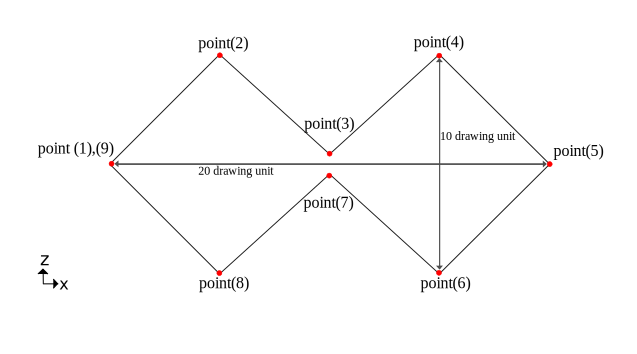
\includegraphics[width=0.8\textwidth]{svg/biquad_prim_curve.pdf}
\caption{Biquad antenna with side length $\sqrt{50}$ in xz-plane.}
\label{fig:primCurve}
\end{figure}

\subsection{Wire} \phantomsection\label{wire}
Introduce a curve with defined radius into \hyperref[CSX]{\matv{CSX}} with matlab function \texttt{AddWire} and assign a property to it. 

\begin{FontNameFunct}{AddWire()}
\end{FontNameFunct}


\begin{FontDescr}{Purpose:}
Add wire to \hyperref[CSX]{\matv{CSX}} by defining its coordinate arrays and radius. Take note that wire is not a solid cylinder!  
\end{FontDescr}

\begin{FontDescr}{Syntax:}
\begin{lstlisting} 
 CSX = AddWire(CSX, propName, prio, points, wire_rad, varargin)
\end{lstlisting}
\end{FontDescr}

\begin{FontDescr}{Description:}

\begin{FontPara}{propName}
Refer to \hyperref[prim_Name]{propName} in \texttt{AddBox}. 
\end{FontPara}

\begin{FontPara}{points}
Refer to parameter \hyperref[points_curve]{\matv{points}} in section \ref{curve}.
\end{FontPara}

\textcolor{varcol}{wire$\_$rad}
\begin{myindentpar}
Wire radius. 
\end{myindentpar}
\end{FontDescr}

\begin{FontDescr}{Optional Arguments:}
The standard trasformation (rotation,translation,scaling) mentioned in  \hyperref[prim_transform]{\matv{'Transform'}} of \texttt{AddBox}.   
\end{FontDescr}

\begin{FontDescr}{Examples:}
\begin{lstlisting} 
%first point
     points(1,1) = 0;points(2,1) = 5;points(3,1) = 0; 
%second point
     points(1,2) = 0;points(2,2) = 5;points(3,2) = 100; 
     CSX = AddMetal(CSX,'metal'); 
     CSX = AddWire(CSX,'metal',10, points,2);
\end{lstlisting}
This example creates a metallic 100 unit long wire.This wire is hollow cylinder with defined radius and very thin shell width.   
\end{FontDescr}


\subsection{Polygon} \phantomsection\label{polygon}
\input{chapter/SEC_CSXCAD_Setup/prim_poly}

\subsection{2D polygon} \phantomsection\label{2dpoly}
\input{chapter/SEC_CSXCAD_Setup/prim_2dpoly}

